\documentclass[10pt,notitlepage,oneside,a4paper]{article}
\usepackage[utf8]{inputenc} 
\usepackage[T1]{fontenc}
\usepackage[spanish]{babel}
\usepackage{datetime} % Personalizar \today
\usepackage{graphicx}
\usepackage{parskip} 
\usepackage{array}
\usepackage{bm} % bold math symbols
%\usepackage{fixltx2e} % \textsubscript y \textsuperscript
\usepackage[a4paper,includeheadfoot,top=1cm,bottom=1cm,left=2cm,right=2cm,head=1.5cm,text=25cm]{geometry} %márgenes
\usepackage{fancyhdr}
\usepackage{fancyvrb}
\usepackage{pstricks}
\usepackage[most]{tcolorbox} % cajas con color de fondo
\usepackage{titlesec}
\usepackage{titletoc}
\usepackage{totpages}
\usepackage{tocloft} % Cambiar aspecto de la tabla de contenidos
\usepackage{siunitx}
\usepackage{booktabs} % Tablas con mejor aspecto
\usepackage{longtable} % tablas que ocupan más de una hoja
\usepackage{enumerate} % http://ctan.org/pkg/enumerate para enumerar con romanos minúsculas
\usepackage{multirow} % http://ctan.org/pkg/multirow
\usepackage[hypcap,font=small,labelfont=bf]{caption} % captionof, con hycap usa la parte superior como referencia
\usepackage{capt-of} % Para usar caption fuera de table o figure (flotados)
\usepackage{float} % posicionamiento H para evitar flotar tablas y figuras
\usepackage[draft,inline,nomargin,lang=spanish,author=]{fixme} % notas
\fxsetup{theme=color}
\usepackage[obeyspaces]{url} %permite espacios en urls
\usepackage[backref,pdfencoding=auto,colorlinks=true,linkcolor=blue]{hyperref}
\usepackage{bookmark} % corrige errores con appendix e hyperref

\renewcommand{\familydefault}{phv} %phv - Helvética para fuente por defecto
\renewcommand{\headrulewidth}{0pt} % Sin línea superior en encabezado
\addto\captionsspanish{\def\tablename{Tabla}} %% Para renombrar cuadros a tablas

\definecolor{block-gray}{gray}{0.95}
\newtcolorbox{myquote}{colback=block-gray,grow to right by=-10mm,grow to left by=-10mm,
boxrule=0pt,boxsep=0pt,breakable}

% Indentados de ToC
\cftsetindents{section}{0em}{5.5em}
\cftsetindents{subsection}{2em}{3.5em}

\setcounter{secnumdepth}{3} %% Hasta que nivel se numeran las secciones
\setcounter{tocdepth}{3} %% Cuantos niveles aparecen en el indice

%% FORMATOS PÁGINA ************************************************************
%% ------------ PÁGINA INICIAL
\makeatletter
\def\ps@portada{%
\def\@oddhead{
\includegraphics[height=1.17cm]{imagenes/mfom}\hfill 
\includegraphics[height=1.17cm]{imagenes/ietcc}~
\includegraphics[height=1.17cm]{imagenes/csic2}}
\def\@evenhead{
\includegraphics[height=1.17cm]{imagenes/mfom}\hfill 
\includegraphics[height=1.17cm]{imagenes/ietcc}~
\includegraphics[height=1.17cm]{imagenes/csic2}}
%\let\@oddhead\@empty%
%\let\@evenhead\@empty%
\def\@oddfoot{\scriptsize\parbox[b]{4cm}{Versión \version ~/ \fecha \\Página~\textbf{\thepage}~de~ \textbf{\ref*{TotPages}}}\hfill
\rule{.2pt}{1.0cm}\quad \parbox[b]{3.5cm}{C/ SERRANO GALVACHE 4\\28033
MADRID ESPAÑA\\TEL: 91 302 04 40\\FAX: 91 302 07 00}
}%
\def\@evenfoot{\scriptsize\parbox[b]{4cm}{Versión \version ~/ \fecha \\Página~\textbf{\thepage}~de~ \textbf{\ref*{TotPages}}}\hfill
\rule{.2pt}{1.0cm}\quad \parbox[b]{3.5cm}{C/ SERRANO GALVACHE 4\\28033
MADRID ESPAÑA\\TEL: 91 302 04 40\\FAX: 91 302 07 00}
}%
}
\makeatother
%% ------------ PÁGINA plain (para ToC)
\fancypagestyle{plain}{%
\fancyhf{} % clear all header and footer fields
\fancyhead[L]{
\includegraphics[height=1.17cm]{imagenes/mfom}}
\fancyhead[R]{\hfill 
\includegraphics[height=1.17cm]{imagenes/ietcc}~
\includegraphics[height=1.17cm]{imagenes/csic2}\\
\scshape \tiny Instituto de Ciencias de la Construcción Eduardo Torroja}
\fancyfoot[L]{\scriptsize\parbox[b]{4cm}{Versión \version ~/ \fecha \\Página~\textbf{\thepage}~de~ \textbf{\ref*{TotPages}}}}
\renewcommand{\headrulewidth}{0pt}
\renewcommand{\footrulewidth}{0pt}
}
%% ------------ PÁGINA TIPO
\pagestyle{fancy}
\fancyhf{}
\lhead{
\includegraphics[height=1.17cm]{imagenes/mfom}}
\rhead{\hfill 
\includegraphics[height=1.17cm]{imagenes/ietcc}~
\includegraphics[height=1.17cm]{imagenes/csic2}\\
\scshape \tiny Instituto de Ciencias de la Construcción Eduardo Torroja
}
\lfoot{\scriptsize \parbox[b]{4cm}{Versión \version ~/ \fecha \\Página~\textbf{\thepage}~de~ \textbf{\ref*{TotPages}}}}
%% FIN FORMATOS ***************************************************************

%% DATOS DEL INFORME **********************************************************
\newcommand{\titulo}{Manual de \texttt{VisorXML}}
\newcommand{\subtitulo}{Visualización y edición de informes de eficiencia energética de edificios para Certificación y verficación del CTE~DB-HE}
\newcommand{\titulocorto}{\titulo} % Título para encabezados
%\newcommand{\tipo}{BORRADOR}%{Documento preliminar} % Tipo documento: PRELIMINAR, FINAL, ETC.
\newdateformat{mydate}{\monthname[\THEMONTH] \THEYEAR}
\newcommand{\fecha}{\mydate\today} % Fecha DD/MM/AAAA o \today para hoy
\newcommand{\version}{1.0}
%% FIN DATOS DEL INFORME ******************************************************

\begin{document}

%% PORTADA *****************************************
\thispagestyle{portada}
\null\vspace{5cm}
%\null\vfill % Usamos párrafo nulo ya que vfill/vspace funciona entre párrafos
\begin{center}
{\Large \bfseries \titulo}
\vskip 0pt\vspace{0.5cm}{\large \subtitulo}
%\vskip 0pt\vspace{0.5cm}{\large \tipo}
\end{center}
%\null\vfill

%% NOTA *****************************************
\null\vfill
%%% AUTORES -----------------------------------------
\begin{center} \footnotesize

\fbox{\parbox{.75\textwidth}{
\textbf{\copyright ~ 2015 Ministerio de Fomento}\\
\textbf{\phantom{\copyright ~ 2015 }Instituto de Ciencias de la Construcción Eduardo Torroja (IETcc-CSIC)}\\[5pt]
\textbf{Autores}:\\[5pt]
\-\qquad Rafael Villar Burke \href{mailto:pachi@ietcc.csic.es}{<pachi@ietcc.csic.es>}\\
\-\qquad Daniel Jiménez González \href{mailto:danielj@ietcc.csic.es}{<danielj@ietcc.csic.es>}
}} %% Nombre de los autores del informe

%\fbox{\parbox{.6\textwidth}{
%\textbf{Nota:}\\[5pt]
%El presente borrador es para uso exclusivo de la persona o entidad a la que está
%dirigido, el receptor le concederá con carácter general la calificación de
%información reservada y restringida.
%
%Los contenidos o ideas recogidas en el mismo pertenecen a sus autores. Se trata
%de un documento preliminar de trabajo y no tiene carácter reglamentario. Los
%autores no se hacen responsables del uso indebido del mismo.
%}} %% Nota

\end{center}
\vskip 0pt\vspace{1.5cm}
\clearpage

\newpage
%% INDICE %%%%%%%%%%%%%%
\tableofcontents
\clearpage

%% DOCUMENTO %%%%%%%%%%%%%%
\newpage
\section{Introducción}

El documento reconocido \href{http://www.minetur.gob.es/energia/desarrollo/EficienciaEnergetica/CertificacionEnergetica/DocumentosReconocidos/Documents/20150625\%20-\%20Informe\%20evaluaci\%C3\%B3n\%20energ\%C3\%A9tica\%20edificio\%20en\%20formato\%20elec\%20XML.pdf}{\textit{Informe de evaluación energética del edificio en formato electrónico (XML)}} recoge la definición de un formato adecuado para la transmisión y almacenamiento electrónico de los datos de la evaluación energética de los edificios orientada a la certificación energética y la verificación del \textit{CTE DB-HE}.

La herramienta web \textit{VisorXML} facilita el manejo de los archivos generados conforme a dicha especificación, con la siguiente funcionalidad:

\begin{itemize}
\item Visualización del \textit{Certificado de eficiencia energética del edificio}
\item Comprobación de la consistencia formal del archivo \texttt{XML} (inclusión de campos obligatorios, tipos de datos correctos, ...), de acuerdo con el esquema \texttt{XSD} publicado
\item Comprobaciones adicionales de consistencia material de los datos del \texttt{XML} (número de plantas, incorporación de archivos de imagen, ...)
\item Generación y descarga del \textit{Certificado de eficiencia energética del edificio} en formato \texttt{PDF}
\item Edición de los campos administrativos del \textit{Certificado de eficiencia energética del edificio} y generación y descarga de los archivos \texttt{XML} y \texttt{PDF} actualizados
\item Incorporación de medidas de mejora energética a un informe \texttt{XML} existente a partir del \texttt{XML} base y otros archivos \texttt{XML} con las medidas de mejora aplicadas
\item Visualización de un informe complementario, orientado a la ayuda al diseño y a la verificación del CTE~DB-HE, permitiendo su descarga en formato \texttt{PDF}
\end{itemize}

\section{Uso de la aplicación}
\label{sec:usoprograma}

\subsection{Organización general de la aplicación}

\textit{VisorXML} es una aplicación web, por lo que, para su utilización, el usuario final solamente necesita disponer de un navegador web\footnote{La aplicación sigue tecnologías web basadas en estándares abiertos por lo que es recomendable el uso de un navegador relativamente reciente \fxnote{Indicar versiones soportadas}.} y acceder al servidor \href{http://146.185.158.142/}{http://146.185.158.142/}\footnote{Dirección web provisional.}.

Además de la pantalla de \textit{Inicio}, la aplicación consta de una pantalla de \textit{Entrada de Datos}, una pantalla de \textit{Certificado de eficiencia Energética}, y una pantalla para el \textit{Informe Complementario}. Se accede a cada una de estas secciones usando una barra de enlaces en la parte superior de la pantalla.

\subsection{Pantalla de Inicio}

Esta pantalla (\autoref{fig:pinicio}) se muestra al abrir la aplicación y al pulsar el enlace \textit{Visor CTE\_XML}, y contiene información general, además de un enlace al archivo de definición del formato \texttt{XML}, al esquema de datos y un par de archivos \texttt{XML} de ejemplo para poder hacer pruebas.

\begin{figure}[H]
  \centering
  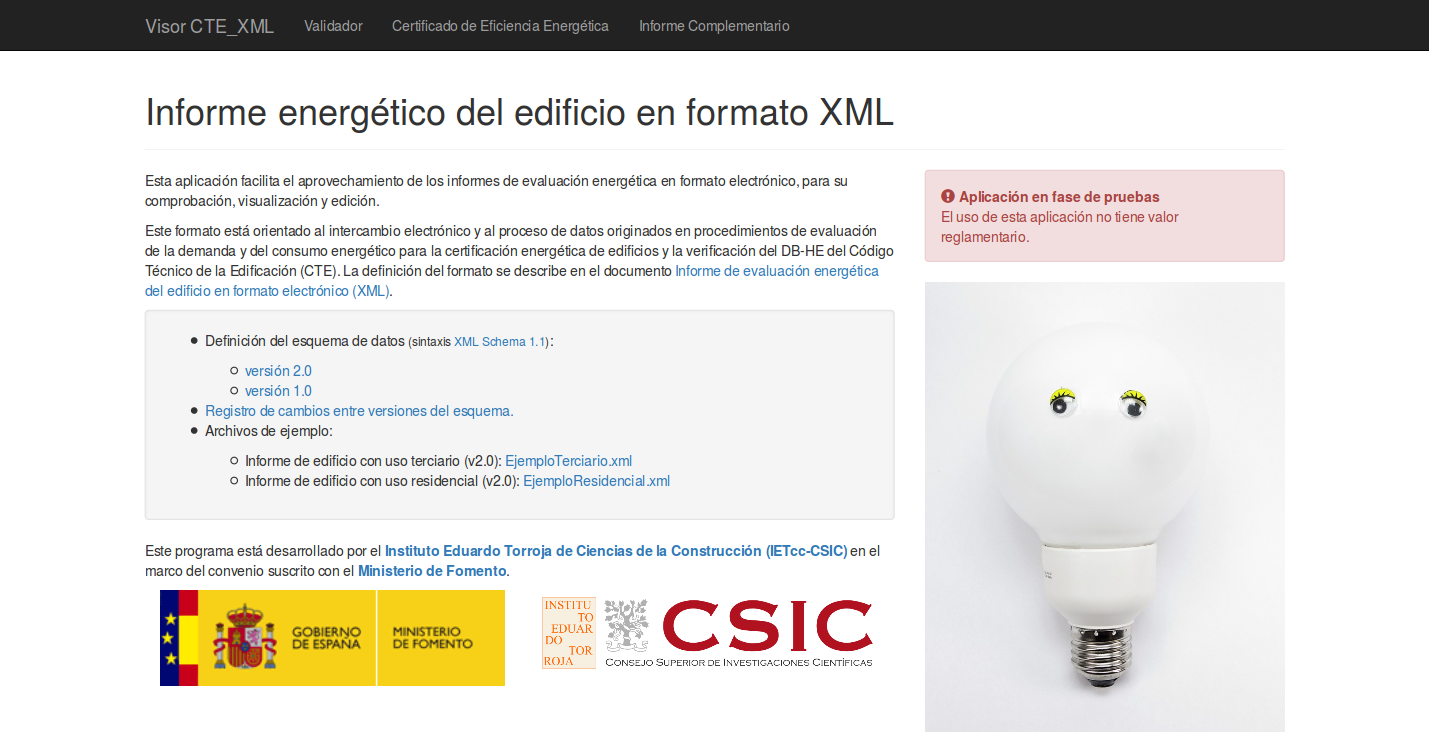
\includegraphics[width=0.75\textwidth]{imagenes/pantalla_inicio}  
  \caption{Pantalla de \textit{Inicio}}
  \label{fig:pinicio}
\end{figure}

\subsection{Entrada de Datos}

Esta pantalla (\autoref{fig:pvalida}) permite subir el archivo \texttt{XML} sobre el que trabajar con la aplicación, así como uno o varios archivos \texttt{XML} que sirven para incorporar medidas de mejora sobre el archivo base.

\begin{figure}[H]
  \centering
  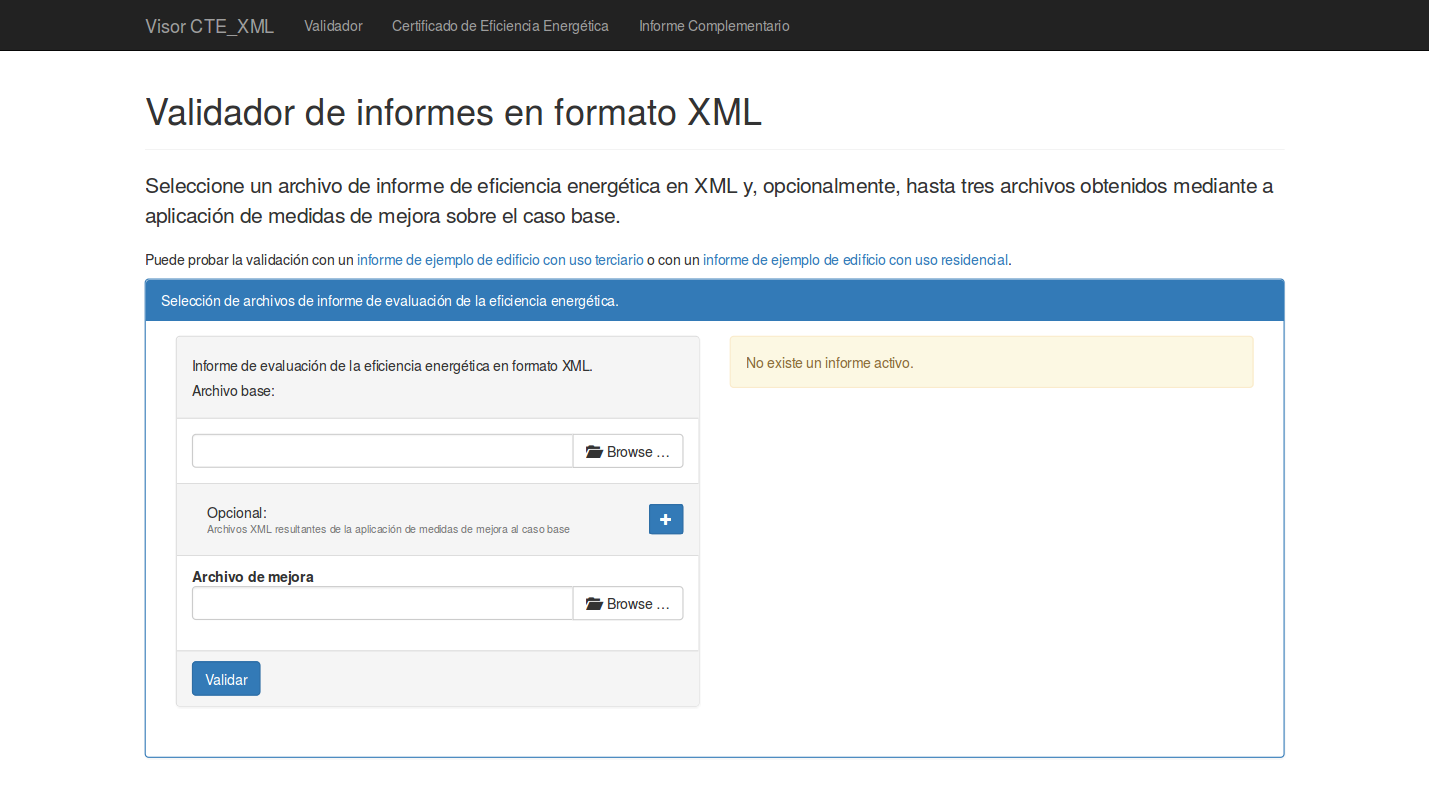
\includegraphics[width=0.75\textwidth]{imagenes/pantalla_entradadatos}  
  \caption{Pantalla de \textit{Entrada de datos}}
  \label{fig:pvalida}
\end{figure}

Al pulsar el botón \textit{"Validar"} en la parte inferior del formulario de entrada de archivos, la aplicación comprueba su contenido, indicando si la validación es correcta (\autoref{fig:pvalidaok}), con un mensaje en un recuadro de color verde.

\begin{figure}[H]
  \centering
  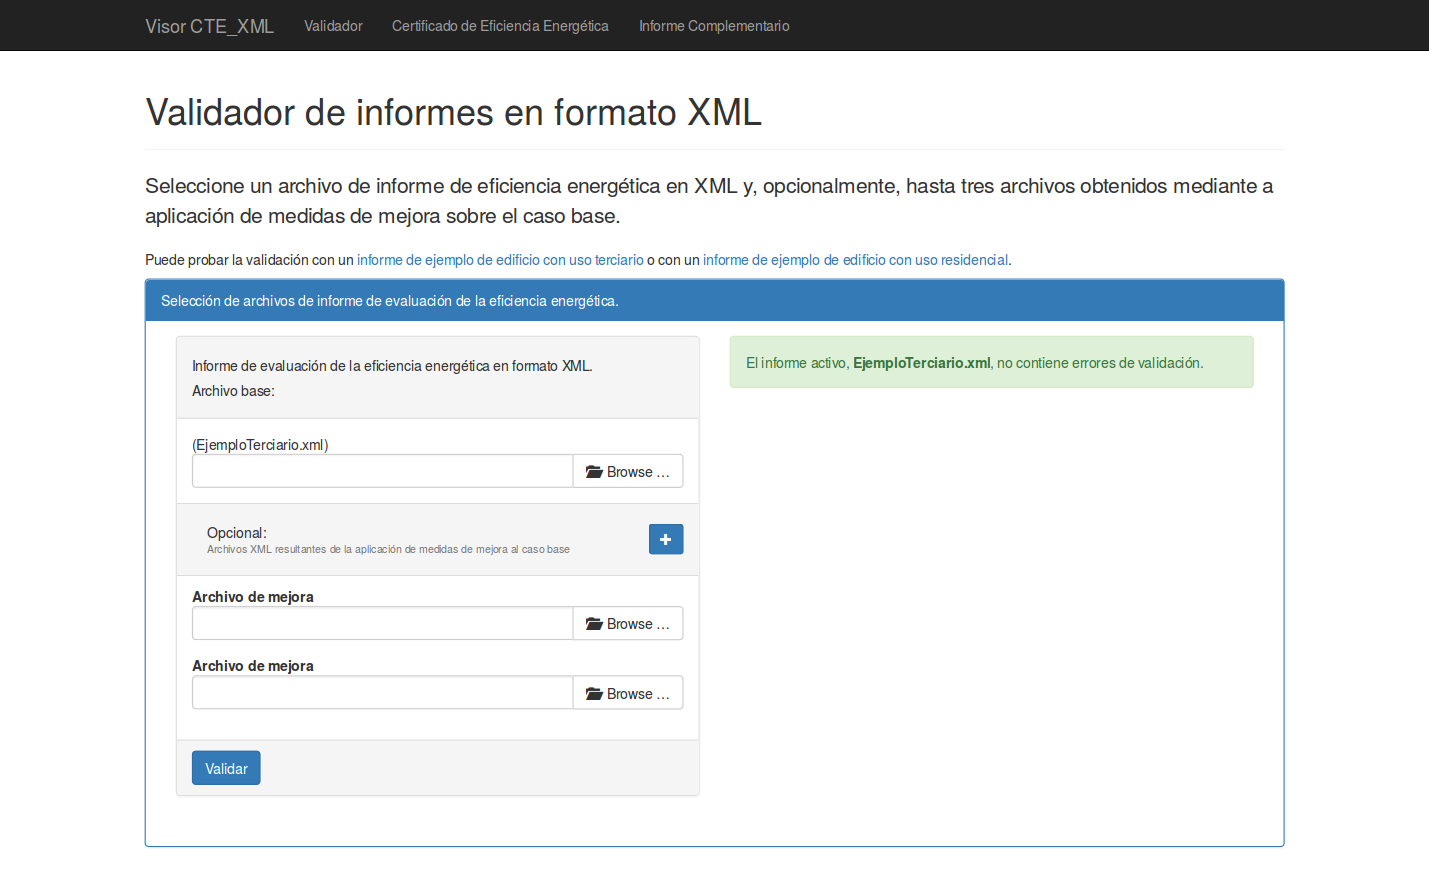
\includegraphics[width=0.75\textwidth]{imagenes/pantalla_entradadatos_validaok}  
  \caption{Pantalla de \textit{Entrada de datos} con validación correcta del archivo \texttt{XML}}
  \label{fig:pvalidaok}
\end{figure}

En caso de que se encuentren valores anómalos o datos inconsistentes, se emiten avisos (\autoref{fig:pvalidaavisos}) en un recuadro de color amarillo. Tanto en este caso, como en el anterior, es posible proceder a la visualización del \textit{Certificado de Eficiencia Energética} o el \textit{Informe Complementario}.

\begin{figure}[H]
  \centering
  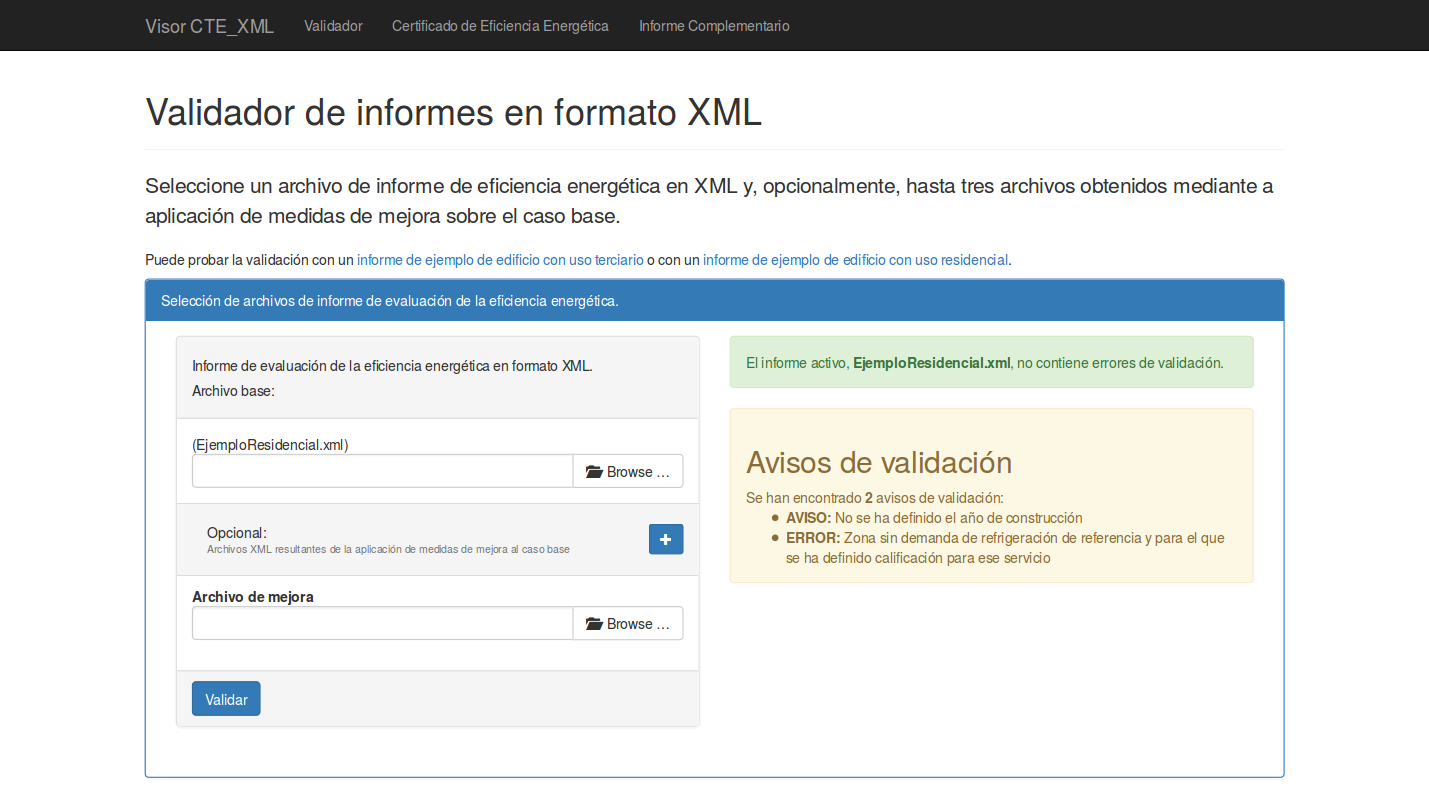
\includegraphics[width=0.75\textwidth]{imagenes/pantalla_entradadatos_validaavisos}  
  \caption{Pantalla de \textit{Entrada de datos} con validación con avisos del archivo \texttt{XML}}
  \label{fig:pvalidaavisos}
\end{figure}

En el caso de que el archivo \texttt{XML} esté mal formado y no responda al esquema \texttt{XSD}, se emiten los errores de validación (\autoref{fig:pvalidaerror}) en un recuadro de color rojo.

\begin{figure}[H]
  \centering
  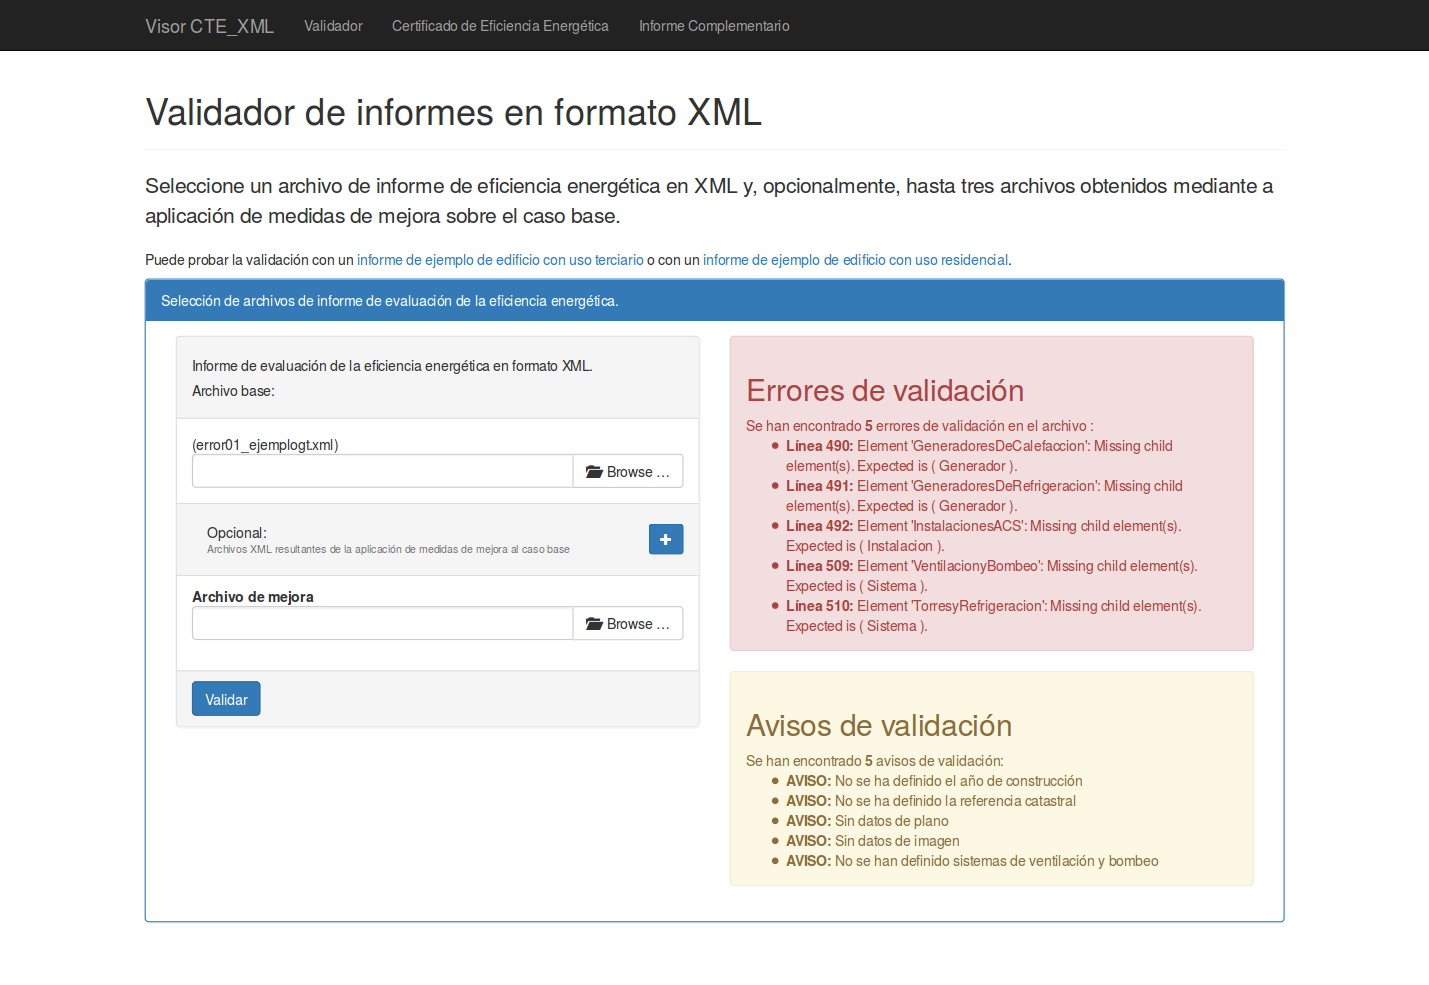
\includegraphics[width=0.75\textwidth]{imagenes/pantalla_entradadatos_validaerror}  
  \caption{Pantalla de \textit{Entrada de datos} con validación errónea del archivo \texttt{XML}}
  \label{fig:pvalidaerror}
\end{figure}

\subsection{Certificado de Eficiencia Energética}

En esta pantalla (\autoref{fig:pcertificado}) se muestra el \textit{Certificado de Eficiencia Energética del Edificio}, generado a partir de los datos del archivo \texttt{XML}.

\begin{figure}[H]
  \centering
  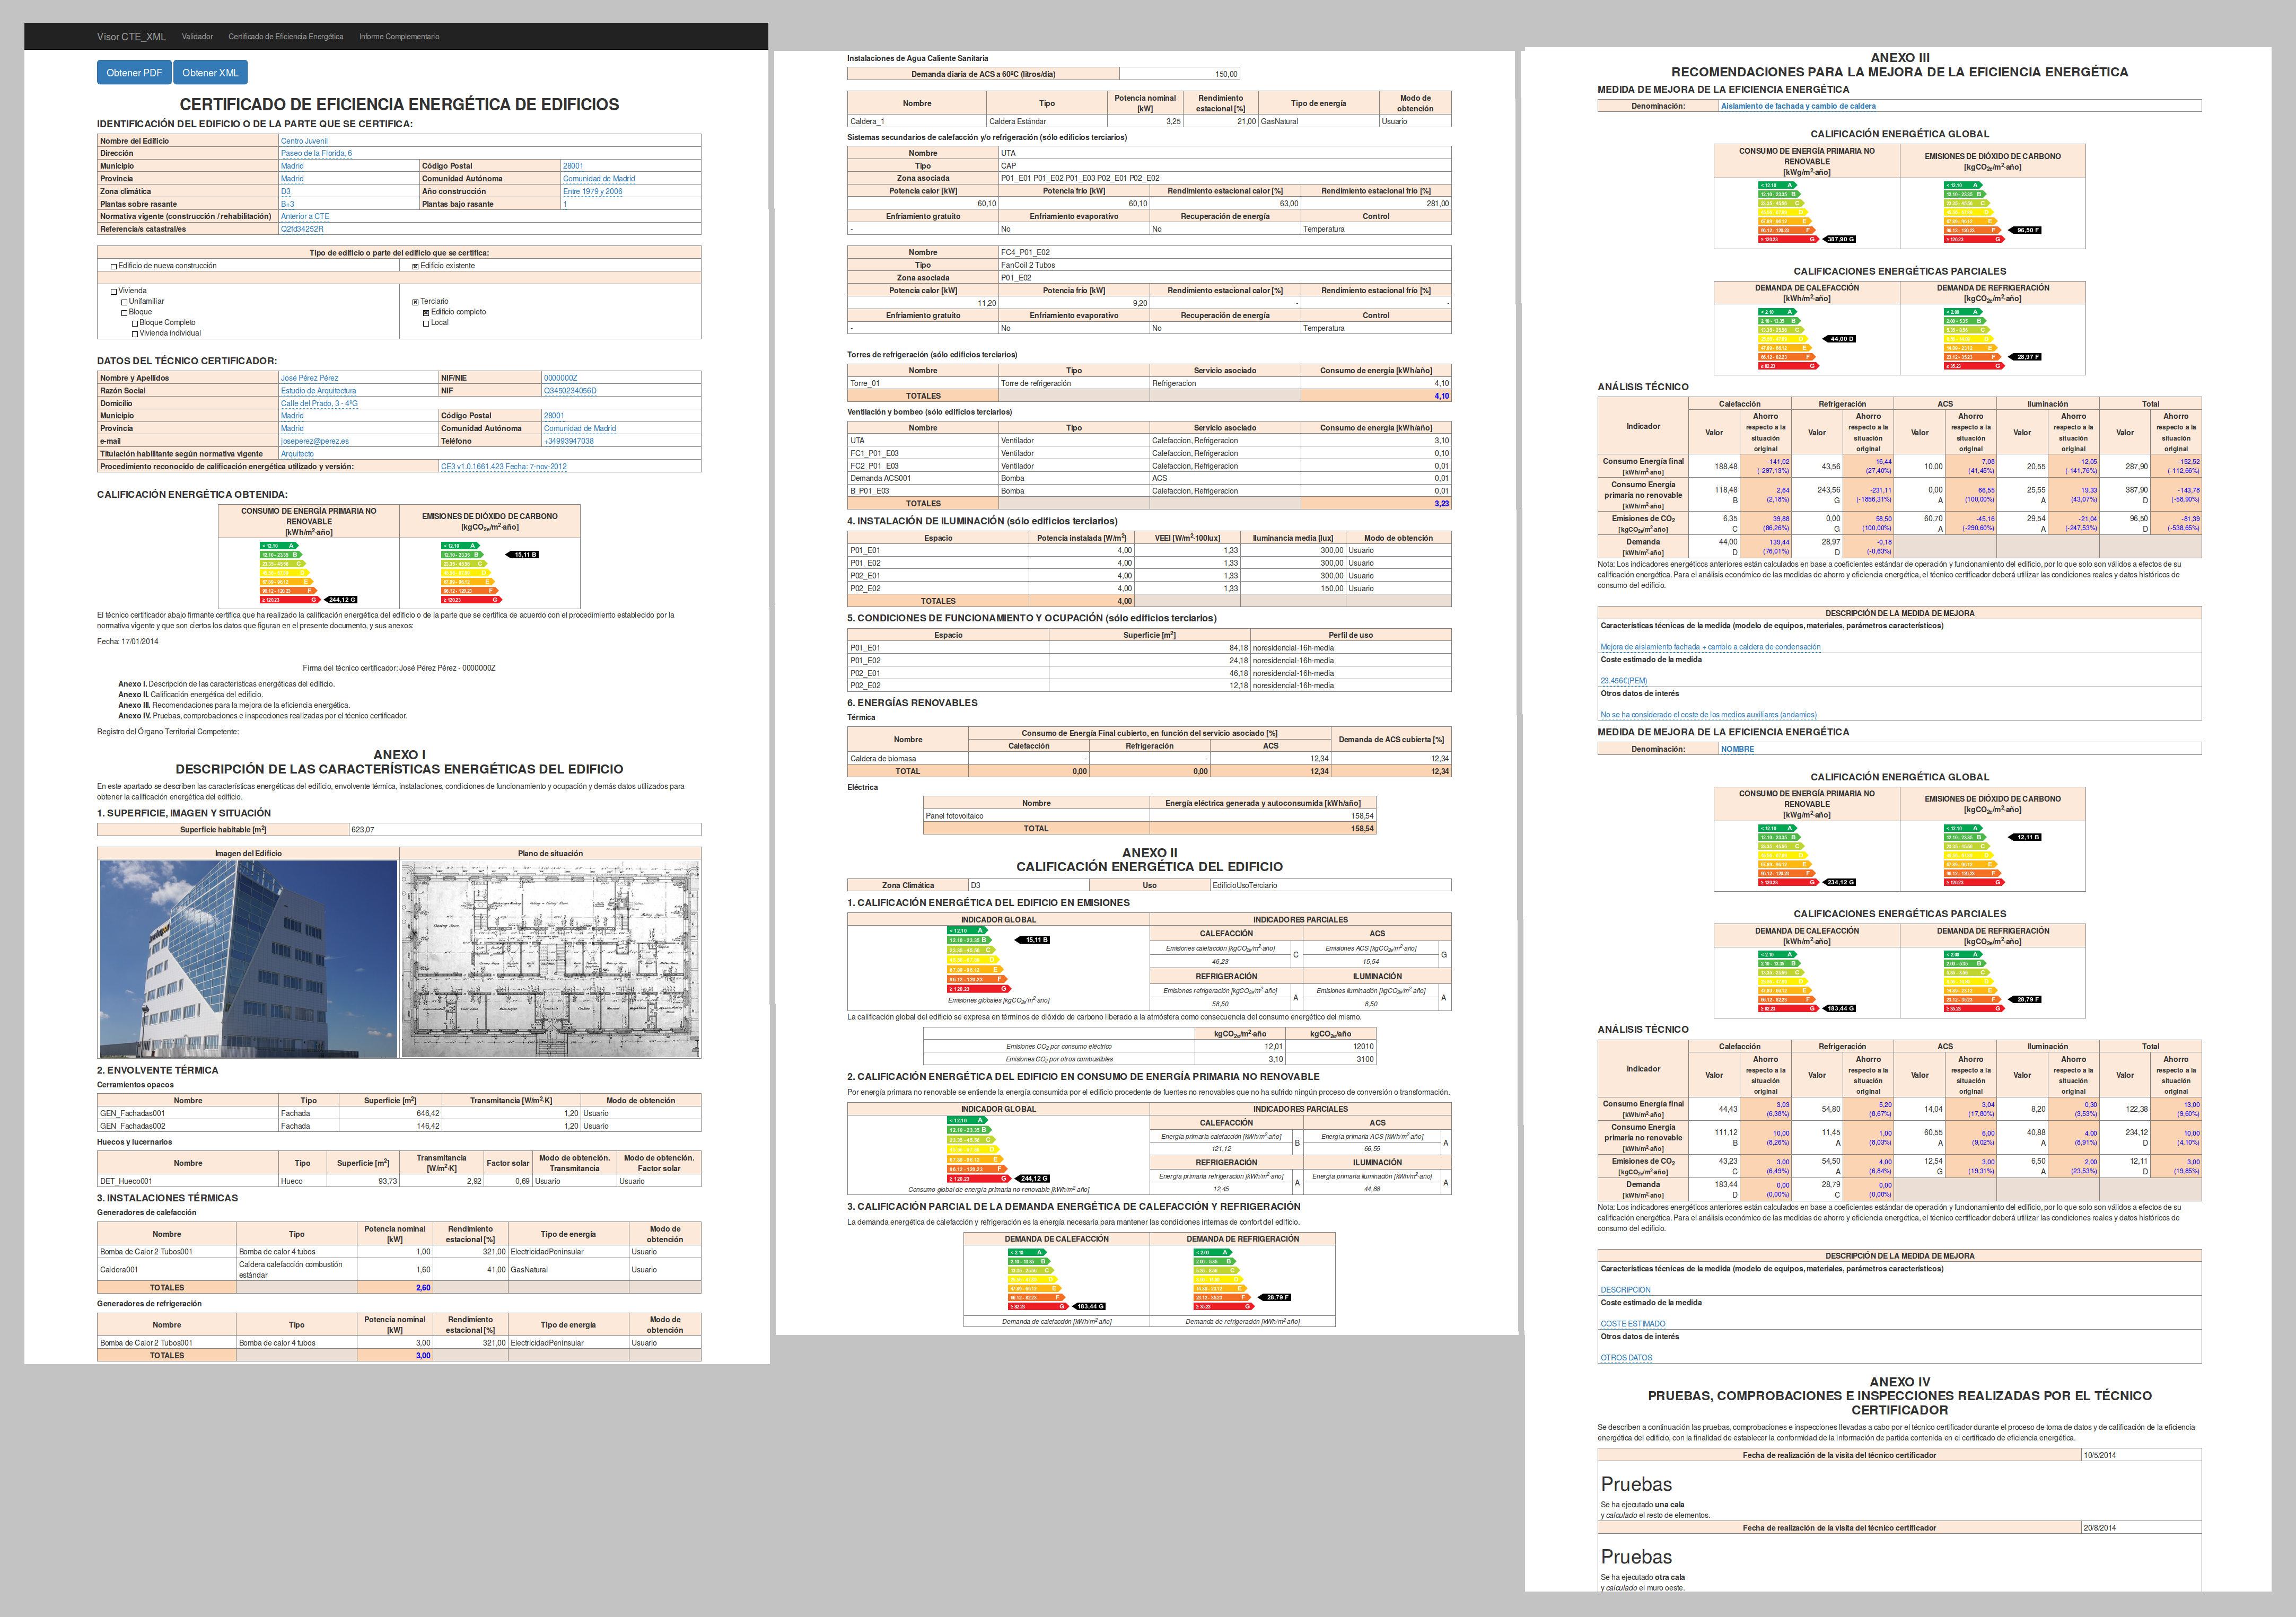
\includegraphics[width=\textwidth]{imagenes/pantalla_certificado_trozos}  
  \caption{Pantalla de \textit{Certificado de Eficiencia Energética}}
  \label{fig:pcertificado}
\end{figure}

Es posible editar parte del documento pulsando sobre los campos que se señalan con un subrayado de líneas azules punteadas, de modo que se activa una casilla de entrada de texto (\autoref{fig:peditacampos}).

\begin{figure}[H]
  \centering
  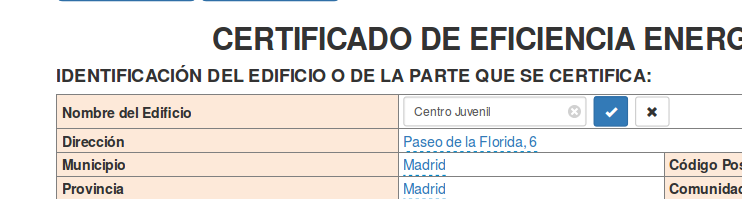
\includegraphics[width=0.75\textwidth]{imagenes/pantalla_editacampos}  
  \caption{Edición en línea de datos administrativos}
  \label{fig:peditacampos}
\end{figure}

Los campos que admiten formato enriquecido del texto se editan igualmente con un editor simple en línea (\autoref{fig:peditarichtext}, \autoref{fig:peditarichtext2}) que incluye la posibilidad de añadir formato al texto (negritas, cursivas, niveles de encabezado, enlaces e imágenes\footnote{En estos momentos la imagen no se archiva en el documento \texttt{XML} descargado}).

\begin{figure}[H]
  \centering
  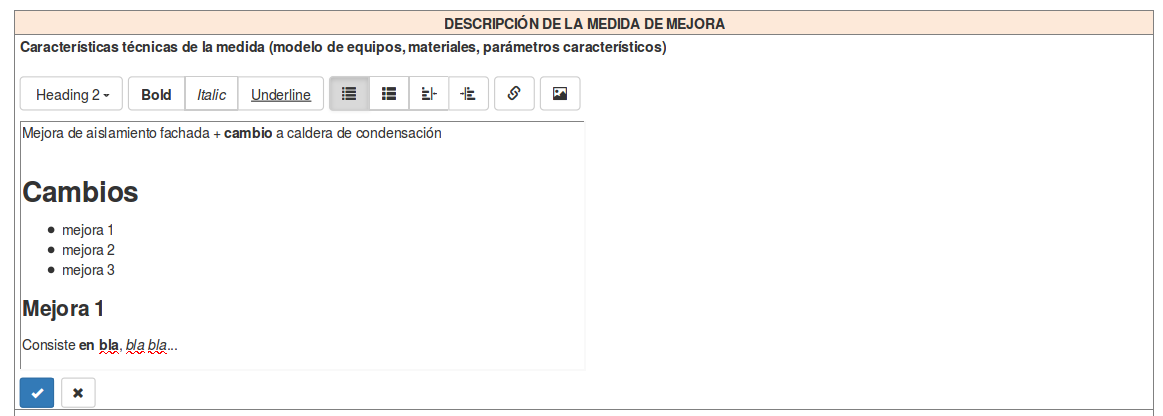
\includegraphics[width=0.75\textwidth]{imagenes/peditarichtext}  
  \caption{Edición enriquecida de datos}
  \label{fig:peditarichtext}
\end{figure}

\begin{figure}[H]
  \centering
  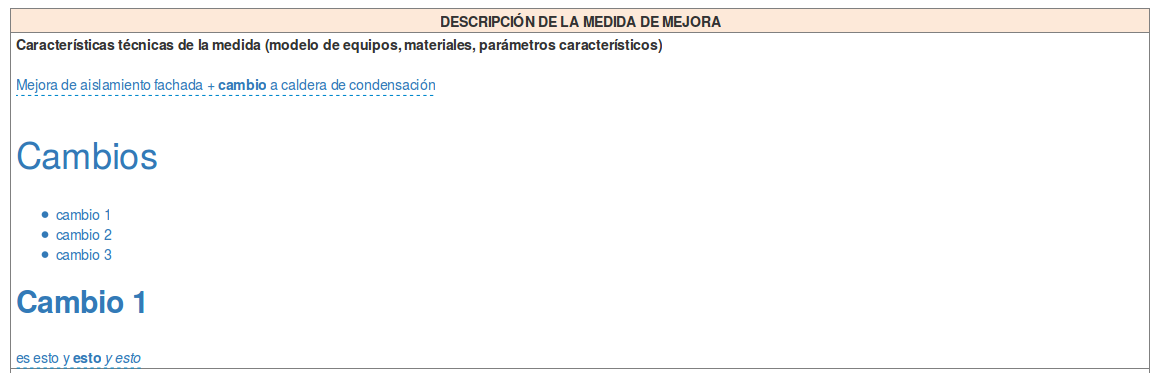
\includegraphics[width=0.75\textwidth]{imagenes/peditarichtext2}  
  \caption{Campo con texto enriquecido}
  \label{fig:peditarichtext2}
\end{figure}

En todo el proceso es posible descargar el documento \texttt{XML} editado o el \texttt{PDF} correspondiente, usando los botones que se sitúan en la parte superior de la pantalla, como se puede ver en la \autoref{fig:pdescargapdf}.

\begin{figure}[H]
  \centering
  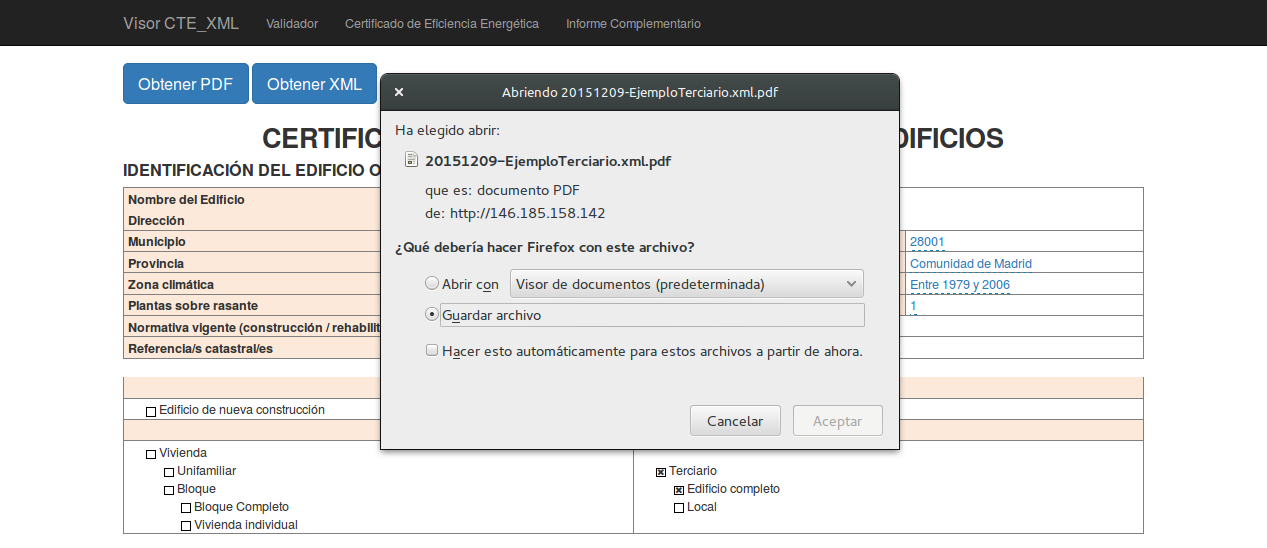
\includegraphics[width=0.75\textwidth]{imagenes/pdescargapdf}  
  \caption{Descarga del \texttt{XML} o del informe en formato \texttt{PDF}}
  \label{fig:pdescargapdf}
\end{figure}

\subsubsection{Introducción de medidas de mejora en el certificado de eficiencia energética}

La certificación energética de edificios exige la definición de medidas de mejora de la eficiencia que se aplican sobre el caso base de estudio. Si bien algunas herramientas gestionan la incorporación de medidas de eficiencia energética, no todas lo permiten.

La aplicación \textit{Visor XML} permite incorporar al archivo \texttt{XML} y, por tanto, al \textit{Certificado de Eficiencia Energética}, medidas de mejora definidas a partir de archivos \texttt{XML} que resultan de la aplicación de medidas de mejora a un modelo energético base.

Para esta funcionalidad es necesario introducir (ver \autoref{fig:pentradamejoras}) el archivo \texttt{XML} del modelo base en la entrada de datos, junto con uno o varios archivos \texttt{XML} obtenidos mediante la aplicación de medidas de mejora al modelo base. El archivo \texttt{XML} base puede contener medidas de mejora definidas con anterioridad en la herramienta de cálculo o a través del propio \textit{Visor XML}.

\begin{figure}[H]
  \centering
  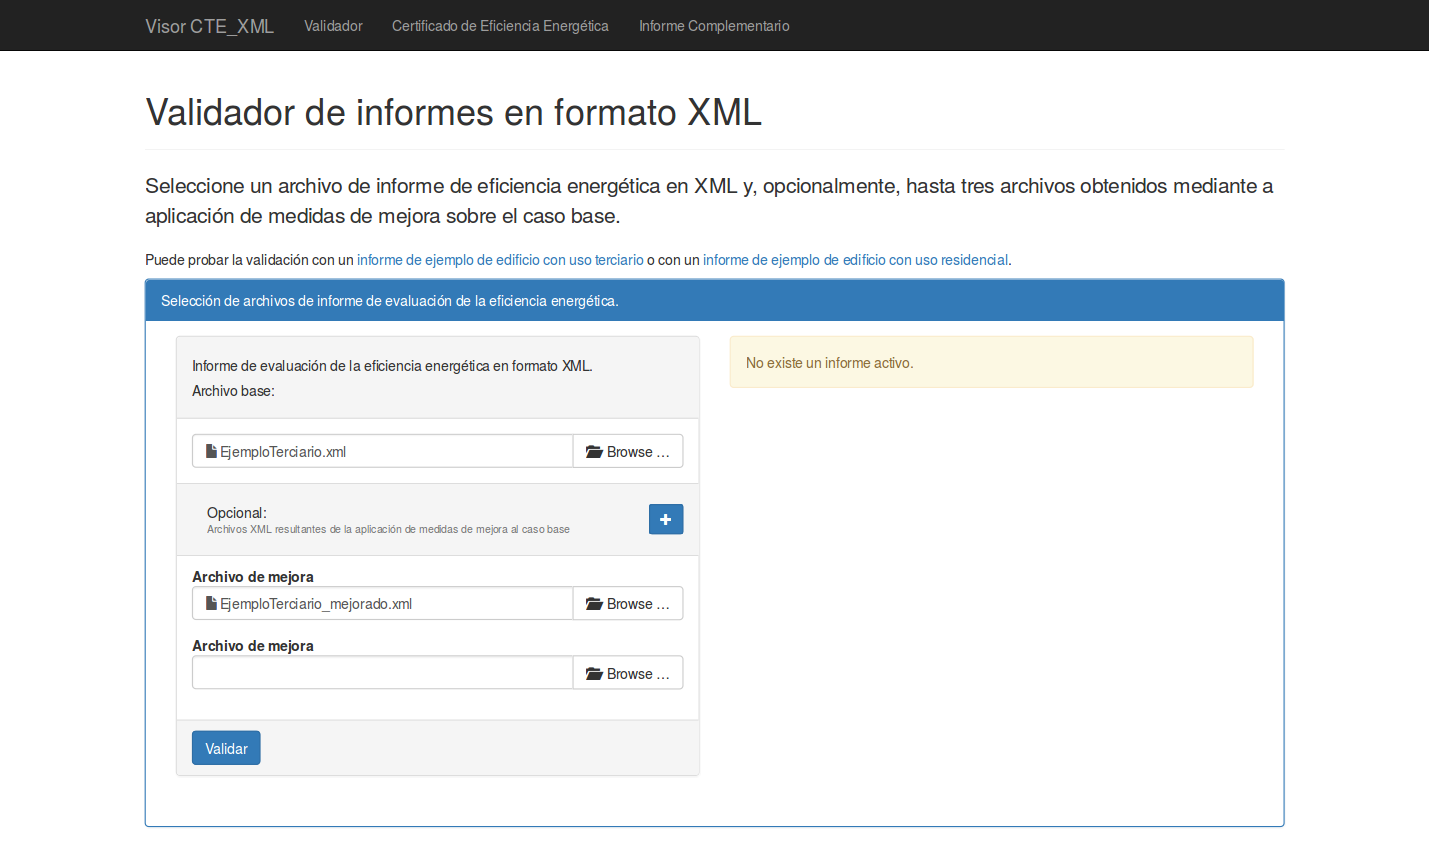
\includegraphics[width=0.75\textwidth]{imagenes/pantalla_entradadatos_mejorado}  
  \caption{Introducción del archivo base y el archivo o archivos con medidas de mejora}
  \label{fig:pentradamejoras}
\end{figure}

Con esto, se incorpora una nueva sección en el anejo de medidas de mejora del \textit{Certificado de Eficiencia Energética} (\autoref{fig:pmedidamejora}) así como la correspondiente información en el archivo \texttt{XML}, pudiendo bajar las versiones modificadas con los botones de descarga.

\begin{figure}[H]
  \centering
  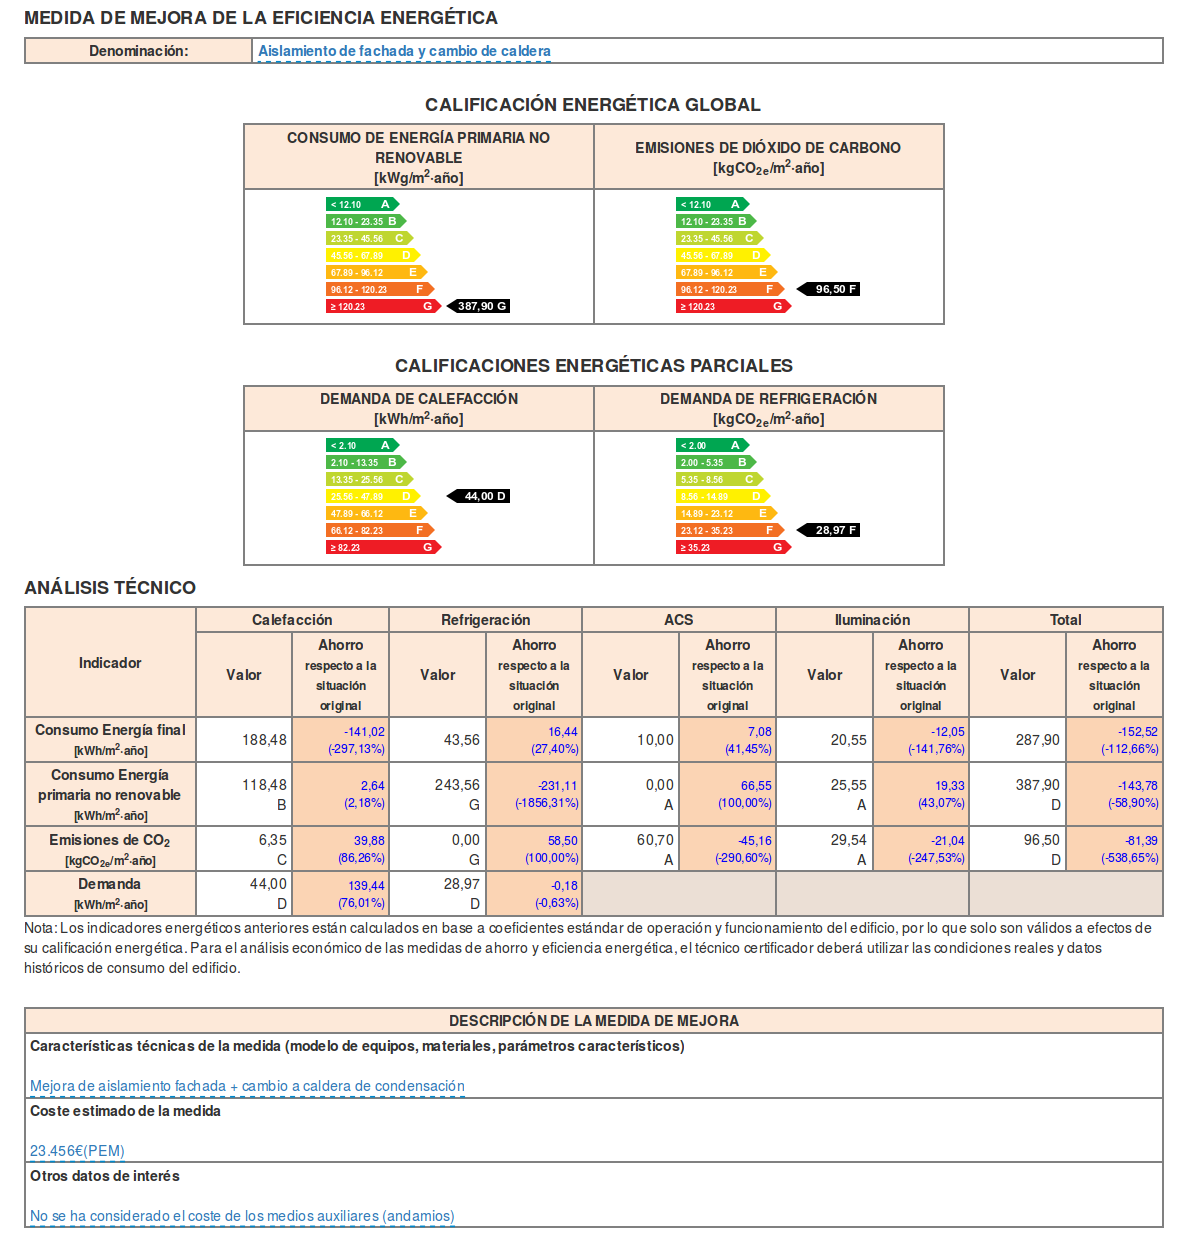
\includegraphics[width=0.75\textwidth]{imagenes/pmedidamejora}  
  \caption{Medida de mejora energética definida a partir de un documento \texttt{XML} complementario al documento \texttt{XML} base}
  \label{fig:pmedidamejora}
\end{figure}

Dado que algunos campos (denominación, características técnicas, coste estimado y otros datos) incluyen información no generada por las herramientas de cálculo, es necesaria su edición por parte del usuario para definir de forma completa la medida de mejora. Para ello basta pulsar con el puntero sobre los campos correspondientes.

\subsection{Informe Complementario}

Además del \textit{Certificado de Eficiencia Energética}, la aplicación \textit{Visor XML} permite visualizar el contenido del archivo \texttt{XML} usando un informe complementario que está orientado a la verificación del \textit{DB-HE} y como ayuda al diseño (\autoref{fig:picomplementario}).

\begin{figure}[H]
  \centering
  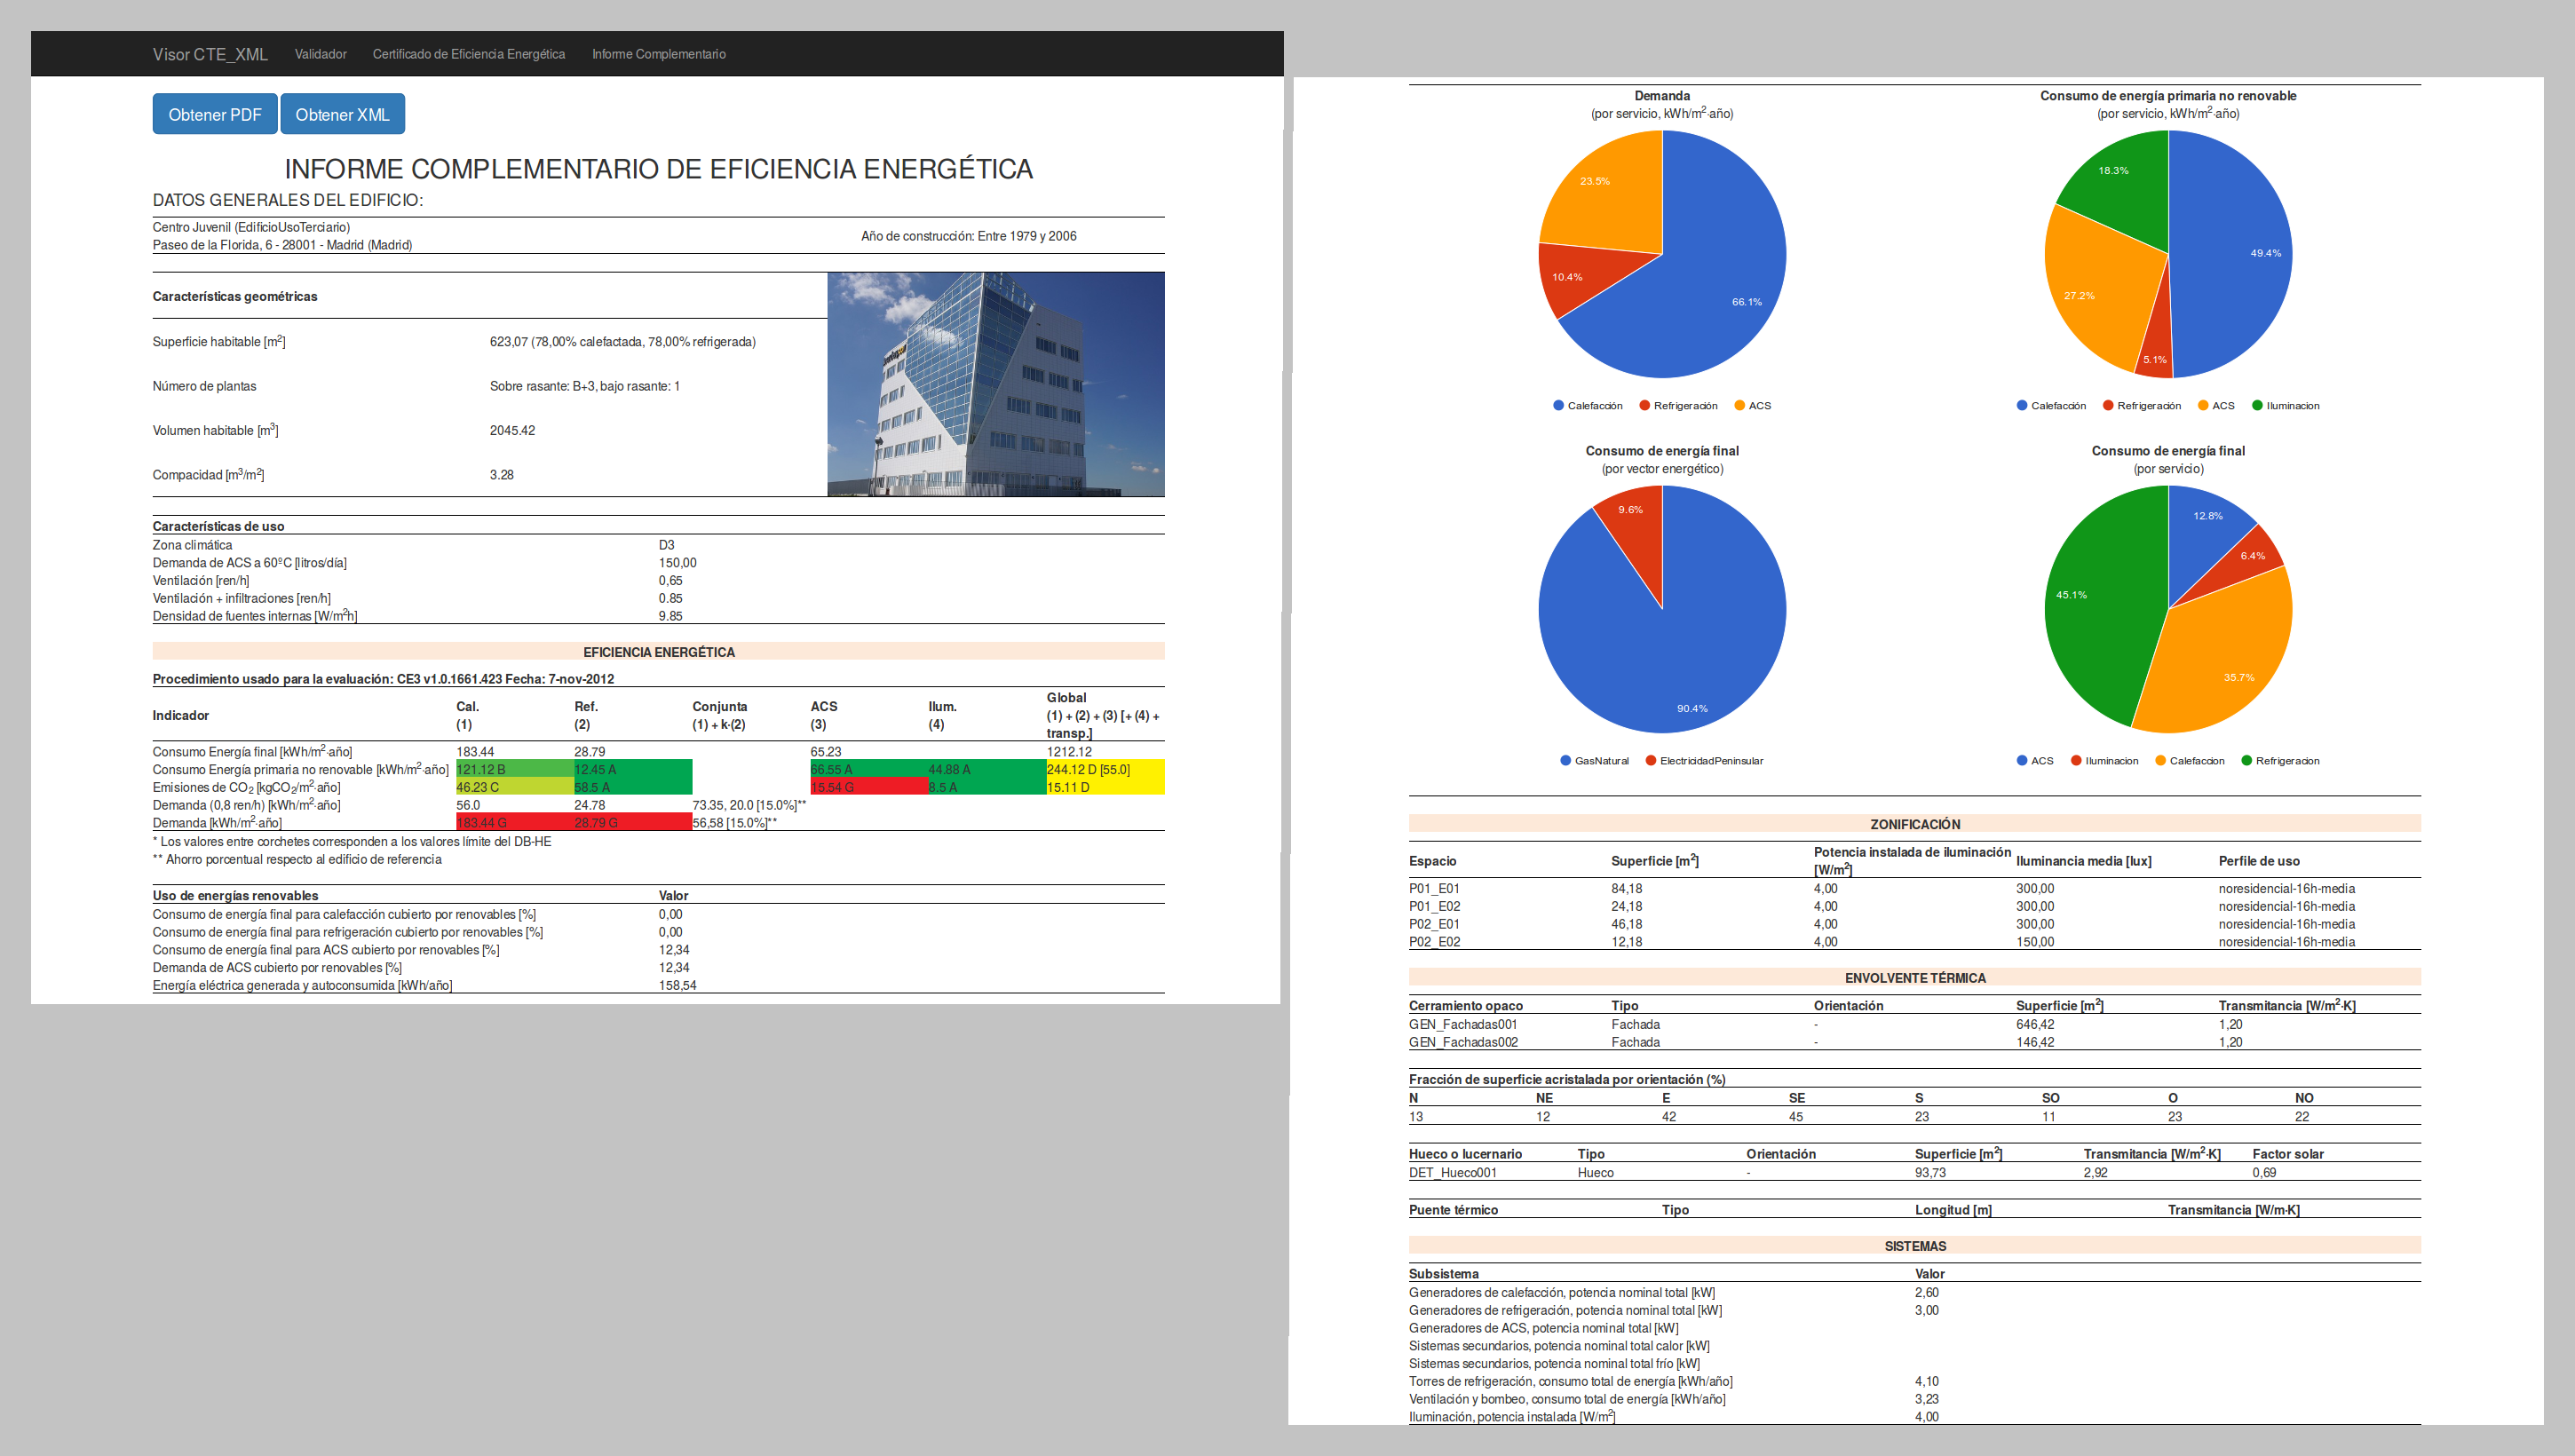
\includegraphics[width=\textwidth]{imagenes/pantalla_informecomplementario_trozos}  
  \caption{Pantalla de \textit{Informe Complementario}}
  \label{fig:picomplementario}
\end{figure}

Además de la identificación del edificio y la información de tipo geométrico (superficies, volumen, compacidad) se aportan datos de condiciones de cálculo (zona climática, nivel de ventilación), principales indicadores y sus referencias normativas (límites normativos señalados entre corchetes, calificación de cada indicador en letra y mediante colores de fondo), o datos de zonficación, envolvente térmica (incluyendo puentes térmicos, si el programa genera estos datos) y sistemas.

El informe incluye también gráficas con la composición por servicios de la demanda y el consumo de energía primaria no renovable y de la composición por servicios y/o vectores energéticos del consumo de energía final.

\section{Mejoras previstas}

A la funcionalidad básica incorporada en la versión original de la aplicación se prevén incorporar nuevas funcionalidades:

\begin{itemize}
\item Generación, lectura y descarga de archivos \texttt{PDF} híbridos (con el documento \texttt{XML} adjunto, de modo que se puede archivar y firmar el conjunto de PDF+XML)
\item Incorporación del \textit{Anejo de justificación de soluciones singulares}, con texto enriquecido
\item Traducción de la interfaz a lenguas cooficiales
\item Mejora del manejo de texto enriquecido (inserción de imágenes)
\item Permitir añadir y eliminar medidas de mejora desde el \textit{Certificado de Eficiencia Energética}, sin necesidad de hacerlo a través de la entrada de datos
\item Permitir la edición, incorporación y eliminación de bloques de \textit{Visitas, inspecciones o comprobaciones}, con botones en línea
\item Comprobaciones de consistencia energética mediante modelo simplificado (aviso si los resultados estimados difieren mucho de los incluidos en el XML)
\item Selección del archivo base \texttt{XML} desde el \textit{Certificado de Eficiencia Energética}, evitando una pantalla adicional de entrada de datos, con cajas de avisos y errores en la misma pantalla
\end{itemize}

Además, podrían resultar interesantes otras funcionalidades para la integración con los registros de certificados:
 
\begin{itemize}
\item Mejoras para la integración con las plataformas informáticas de los registros
\item Sistema de firma y y envío a los registros (con incorporación de formularios adicionales para datos administrativos, etc) de los documentos PDF+XML
\item Muestra de datos estadísticos al usuario (percentil de consumo y demanda del certificado entregado)
\item Panel de gestión para los registros, con posibilidad de incorporar información adicional, gestión de archivos PDF+XML, visualización de informes, etc
\end{itemize}

\section{Tecnologías utilizadas}

La aplicación \textit{VisorXML} es un desarrollo basado en software libre, que se publica bajo una licencia libre (\textit{MIT}), y que emplea las siguientes tecnologías:

\textbf{Gestión del código}

\begin{itemize}
\item Control de versiones con \texttt{git}
\item Repositorio en \texttt{github}
\item Gestión de software con \texttt{Bower} + \texttt{NodeJS}
\item Automatización de despliegue: \texttt{Grunt} + \texttt{pip}
\end{itemize}

\textbf{Backend}

\begin{itemize}
\item Desarrollo en lenguaje \texttt{Python}
\item \texttt{Django} (prototipo inicial en \texttt{Flask})
\item \texttt{lxml}
\item \texttt{Pillow}
\item Impresión \texttt{PDF} con \texttt{PhantomJS}
\end{itemize}

\textbf{Frontend}

\begin{itemize}
\item \texttt{HTML} + \texttt{CSS} + \texttt{JavaScript}
\item \texttt{Bootstrap 3} + \texttt{Bootstrap-fileinput}
\item \texttt{jQuery}
\end{itemize}

La estructura del código es la reflejada en la \autoref{fig:estructuracodigo}:

\begin{figure}[H]
  \centering
  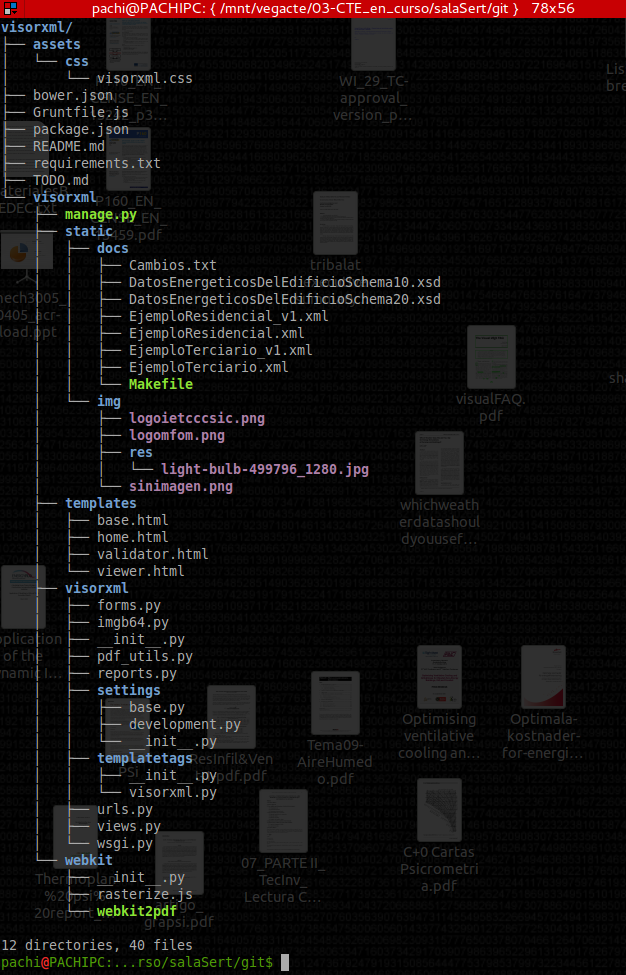
\includegraphics[width=0.5\textwidth]{imagenes/visorxml_estructura}  
  \caption{Estructura de archivos del proyecto \textit{Visor XML}}
  \label{fig:estructuracodigo}
\end{figure}

En el documento \texttt{README.md} se incluyen instrucciones para la instalación de la aplicación en un servidor \textit{GNU/Linux} con \textit{Apache}.
\end{document}
